\documentclass[12pt,a4paper]{article}
\usepackage[utf8]{inputenc}
\usepackage[T1]{fontenc}
\usepackage[spanish,es-tabla]{babel}
\usepackage{graphicx}
\usepackage{float}
\usepackage{geometry}
\usepackage{hyperref}
\usepackage{fancyhdr}
\usepackage{titlesec}
\usepackage{booktabs}
\usepackage{array}
\usepackage{longtable}
\usepackage[table]{xcolor}
\usepackage{mathptmx}
\usepackage{amsmath}
\usepackage{enumitem}
\setlist{itemsep=1pt,topsep=3pt,parsep=0pt}
\setlength{\belowcaptionskip}{4pt}
\usepackage{setspace}
\usepackage{xurl}

\geometry{top=2.5cm, bottom=2.5cm, left=3cm, right=3cm}
\hypersetup{colorlinks=true, linkcolor=black, urlcolor=blue, citecolor=black}
\graphicspath{{data/}{outputs/}}

% bloque "Cómo leerla" de figuras y tablas de resultados
\newcommand{\comoleerla}[3]{%
  \begin{center}\footnotesize
  \begin{minipage}{0.94\linewidth}
  \begin{itemize}\setlength{\itemsep}{0pt}\setlength{\topsep}{2pt}%
    \setlength{\parsep}{0pt}
  \item \textbf{Estructura:} #1
  \item \textbf{Qué se ve:} #2
  \item \textbf{Por qué:} #3
  \end{itemize}
  \end{minipage}
  \end{center}}

\pagestyle{fancy}
\fancyhf{}
\fancyhead[L]{\small Formulación Corte 1: red de carga interurbana}
\fancyhead[R]{\thepage}
\renewcommand{\headrulewidth}{0.4pt}
\setlength{\headheight}{14.5pt}
\setlength{\emergencystretch}{3em}

\titleformat{\section}{\normalfont\Large\bfseries}{\thesection}{1em}{}
\titleformat{\subsection}{\normalfont\large\bfseries}{\thesubsection}{1em}{}
\titleformat{\subsubsection}{\normalfont\normalsize\bfseries}{\thesubsubsection}{1em}{}

\begin{document}

\begin{titlepage}
\thispagestyle{empty}
\centering

\vspace*{0.5cm}

\includegraphics[width=0.30\textwidth]{sergio_logo.png}\\[0.4cm]

{\fontsize{13}{15}\selectfont\textbf{UNIVERSIDAD SERGIO ARBOLEDA}}\\[2.0cm]

{\fontsize{14}{17}\selectfont\textbf{FORMULACIÓN DEL PROBLEMA Y AGENTE DE RUTAS\\
PARA UNA RED DE CARGA INTERURBANA}}\\[0.6cm]
{\fontsize{12}{14}\selectfont Proyecto Integrador, Corte 1}\\[2.5cm]

{\fontsize{12}{14}\selectfont\textbf{Inteligencia Artificial (SIST5036)}}\\[1.5cm]

{\fontsize{12}{14}\selectfont
Juan David Andradé Gómez\\[0.2cm]
Mario Jiménez López\\[0.2cm]
Camilo Andrés Díaz García}\\[1.2cm]

{\fontsize{12}{14}\selectfont Profesor: Joaquín F. Sánchez}

\vfill

\begin{center}
    \textit{Universidad Sergio Arboleda}\\
    \textit{Facultad de Sistemas e Ingeniería}\\
    \textit{Bogotá D.C., 2026}
\end{center}

\end{titlepage}

\newpage
\tableofcontents
\newpage

\section{Descripción del problema}

Un camión de carga de categoría III (dos ejes) debe desplazarse entre
ciudades de Colombia por la red vial nacional. Cada tramo entre dos ciudades
tiene tres magnitudes: la distancia en kilómetros, el costo de peaje en pesos
colombianos (COP) y el riesgo de siniestralidad de la vía. El agente recibe
una ciudad de origen, una de destino y un criterio, y devuelve la ruta de
menor costo según ese criterio. Además de esas magnitudes, el agente calcula
el costo en pesos del trayecto: el peaje más el combustible, que se obtiene de
la distancia, el precio del galón de ACPM y el consumo de un camión de dos
ejes (sección del costo monetario).

La red modelada tiene 32 ciudades y 32 tramos (Tabla~\ref{tab:estadisticas}).
Es un grafo no dirigido, conexo y con exactamente un ciclo independiente
($E-V+1=1$). Ese ciclo, que cierra por Santander, permite que algunos pares
de ciudades tengan dos rutas reales distintas.
El caso de referencia es Duitama a Puente Nacional: 309.10 km por Bogotá o 654.25 km por Santander (con las distancias sin corregir, 414.84 y 668.14 km).


\section{Modelo PEAS}

\begin{table}[H]
\centering
\caption{Modelo PEAS del agente de rutas}
\label{tab:peas}
\renewcommand{\arraystretch}{1.2}
\begin{tabular}{|l|>{\raggedright\arraybackslash}p{10cm}|}
\hline
\rowcolor{gray!20} \textbf{Componente} & \textbf{Definición} \\
\hline
\textbf{Performance} & Minimizar el costo compuesto (distancia, peaje, riesgo), el costo en pesos (peaje más combustible) y responder en tiempo útil \\
\hline
\textbf{Environment} & Red vial interurbana de 32 nodos y 32 aristas, estática, determinista, discreta y totalmente observable \\
\hline
\textbf{Actuators} & Elegir el siguiente tramo de carretera \\
\hline
\textbf{Sensors} & Posición actual (ciudad) y estado de los tramos disponibles (grafo persistido) \\
\hline
\end{tabular}
\end{table}

El entorno es estático (los tramos y sus valores no cambian durante la
consulta), determinista (la misma consulta produce la misma ruta), discreto
(ciudades y tramos finitos) y totalmente observable (el grafo completo está
disponible para el agente).

\section{Datos y metodología de cruce}

Los tres conjuntos provienen del portal de datos abiertos del Estado
colombiano y se descargaron el 6 de octubre de 2026 por la API Socrata. Su
verificación contra la fuente (filas, columnas y hash) está en
\texttt{data/carga/VERIFICACION.md}.

\begin{table}[H]
\centering
\caption{Fuentes de datos (versión del 6 de octubre de 2026)}
\label{tab:fuentes}
\renewcommand{\arraystretch}{1.2}
\begin{tabular}{|l|l|c|r|}
\hline
\rowcolor{gray!20} \textbf{Conjunto} & \textbf{Entidad} & \textbf{Identificador} & \textbf{Filas} \\
\hline
\textbf{Red Vial} & INVÍAS & \texttt{ie7y-asdn} & 715 \\
\hline
\textbf{Peajes} & INVÍAS & \texttt{68qj-5xux} & 179 \\
\hline
\textbf{Sectores críticos de siniestralidad vial} & ANSV & \texttt{rs3u-8r4q} & 316 \\
\hline
\end{tabular}
\end{table}

Para los datos que esos tres conjuntos no traen se evaluaron fuentes
adicionales (el detalle, con la decisión sobre cada una, está en
\nolinkurl{data/carga/FUENTES\_NUEVAS.md}). Cuatro se aceptaron y entran al
modelo (Tabla~\ref{tab:fuentes-comp}).

\begin{table}[H]
\centering
\caption{Fuentes complementarias aceptadas (consulta del 8 de octubre de 2026)}
\label{tab:fuentes-comp}
\renewcommand{\arraystretch}{1.2}
\begin{tabular}{|>{\raggedright\arraybackslash}p{4.6cm}|>{\raggedright\arraybackslash}p{3.2cm}|>{\raggedright\arraybackslash}p{5.6cm}|}
\hline
\rowcolor{gray!20} \textbf{Fuente} & \textbf{Entidad} & \textbf{Uso en el modelo} \\
\hline
\textbf{Red Vial, progresivas del sector} (\texttt{ie7y-asdn}) y \textbf{Postes de Referencia} (\texttt{ufg7-is7r}, 17\,816 filas) & INVÍAS & Distancia de Chocontá a Tunja (61.0 km) \\
\hline
\textbf{Precios de combustibles líquidos} & CREG & Precio del galón de ACPM: 11\,320 COP \\
\hline
\textbf{Línea base de consumo de combustible de vehículos de carga} & UPME & Consumo del camión de dos ejes: 38.69 litros por 100 km \\
\hline
\textbf{Sectores críticos de mortalidad 2022} (\texttt{ybqk-8s42}, 647 filas) & ANSV & Atributo de riesgo adicional y variante de sensibilidad; no es la base \\
\hline
\end{tabular}
\end{table}

Las otras fuentes evaluadas (fletes y costos del RNDC y del SICE-TAC,
homicidios en accidentes de tránsito de la Policía Nacional, estado de las
vías, tráfico vehicular, sectores críticos por exceso de velocidad y
coordenadas de los tres nodos sin punto DANE) se rechazaron o no tienen datos
descargables; ninguna cambia la red.

Cada atributo de arista se obtiene así:

\begin{itemize}
\item \textbf{Distancia.}
\begin{itemize}
\item Se cruza por el texto exacto del campo \texttt{sector} de la Red Vial, no
por \texttt{codigo\_tramo}, porque un mismo código agrupa subtramos de longitud
distinta. Con el código se asignaba la misma longitud a subtramos diferentes
(error real detectado y corregido).
\item Cuando un sector tiene registros duplicados se toma la longitud máxima.
\item En los registros de doble calzada digitalizada se usa el tramo entre
progresivas en lugar de la longitud registrada (ver la sección de auditoría
geométrica).
\item Para Chocontá a Tunja el sector registrado está truncado (17.69 km);
se usa la diferencia de progresivas oficiales entre los dos sectores de la
misma ruta y el mismo tramo (61.0 km), con la condición de que no sea menor
que la distancia geodésica entre los nodos (56.96 km). La longitud registrada
se conserva como variante de sensibilidad.
\end{itemize}
\item \textbf{Peaje.} Para cada arista se identificó a mano el peaje de
INVÍAS ubicado sobre ese subtramo. La tarifa de categoría III se lee de
\texttt{peajes.csv}, mediante una tabla explícita entre el peaje del grafo y
su fila (nombre y código del peaje); el programa falla si un peaje no aparece
exactamente una vez.
\item \textbf{Riesgo.} El conjunto de siniestralidad no indica el subtramo,
solo el corredor. Por eso el riesgo se asigna por corredor completo: puntaje
GiZScore promedio, fallecidos históricos y número de puntos críticos. Como
atributo adicional se cruzaron, por geometría (extremos a no más de 0.3 km del
trazado de la arista), los sectores críticos de mortalidad de la ANSV; 16 de
las 32 aristas tienen al menos un sector. Ese atributo no reproduce el orden
del puntaje GiZScore en las 11 aristas que tienen ambos (correlación de
Spearman $-0.033$) y solo trae sectores de alta prioridad, de modo que se usa
únicamente como variante de sensibilidad.
\end{itemize}

Cinco hechos de los datos condicionan el modelo:

\begin{itemize}
\item \textbf{San Gil a Bucaramanga.} Figura en la Red Vial en dos registros
con progresivas complementarias (82.95 km y 26.19 km), no como duplicado de
calzada, por lo que se suman. Es la única arista donde se suman registros en
vez de tomar el mayor. Con la regla de doble calzada, el registro de 26.19 km
pasa a 12.30 km y la arista queda en 95.25 km.
\item \textbf{Bogotá a Villeta: artefacto de doble calzada digitalizada.} La
fuente reporta 167.67 km para ese sector, cerca del doble de su tramo entre
progresivas (81.00 km), porque su geometría contiene ambas calzadas. La
corrección aplicada deja 81.00 km.
\item \textbf{Chocontá a Tunja: sector truncado.} El sector de la Red Vial
registra 17.69 km, pero Chocontá queda a 43.70 km de su geometría. Las
progresivas oficiales del corredor (Chocontá en PR 59.0 y Tunja en PR 120.0,
ruta 55, tramo 5501) dan 61.0 km, y esa es la distancia de la arista.
\item \textbf{Exclusión de una rama.} Se excluyó la rama Villavicencio,
Barranca de Upía y Yopal por no existir un tramo verificable que conecte
Barranca de Upía con Yopal.
\item \textbf{Exclusión de Mosquera.}
\begin{itemize}
\item La arista de Bogotá a Mosquera usaba el sector Puente Mosquera a Cruce
Avenida del Ferrocarril, que pertenece a la Troncal del Eje Cafetero, a unos
160 km de Mosquera (Cundinamarca), y la Red Vial no tiene un sector oficial de
reemplazo.
\item Como Mosquera era una hoja (solo conectaba con Bogotá), se excluyó el
nodo con su arista, con el mismo criterio que la rama anterior: sector de otra
región y sin sector oficial de reemplazo.
\item La red pasó de 33 a 32 nodos y de 33 a 32 aristas.
\end{itemize}
\end{itemize}

\subsection{Hallazgo del barrido de ciclos}

\textbf{Punto de partida.} La primera versión de la red tenía 27 nodos y 26
aristas, es decir, un árbol: entre dos ciudades cualesquiera existe una única
ruta posible.

\textbf{Revisión.} Se revisaron los 714 segmentos de la Red Vial vigentes al
inicio del trabajo, normalizando los nombres de los sitios. En el alcance
regional original (Cundinamarca, Boyacá, Meta y Tolima), la red troncal
resultó ser un árbol.

\textbf{Resultado.} El único ciclo real que toca los nodos del proyecto cierra
por Santander; se incorporó con seis nodos nuevos (San Gil, Bucaramanga,
Cuestaboba, Pamplona, Presidente y La Palmera) y siete aristas, todas
verificables en el mismo conjunto de datos.

\section{Red y estadísticas}

\textbf{Mapa.} La Figura~\ref{fig:red} muestra la red sobre coordenadas
geográficas, con el trazado de INVÍAS de cada tramo; donde la geometría no
llega al nodo, una línea punteada recta lo une con el extremo del trazado.

\textbf{Ciclo.} El ciclo, en azul, pasa por Cajicá, Bogotá, Tocancipá,
Chocontá, Tunja, Duitama, La Palmera, Presidente, Pamplona, Cuestaboba,
Bucaramanga, San Gil, Puente Nacional, Ubaté y Zipaquirá.

\textbf{Detalle de las aristas.} El detalle de las 32 aristas (distancia,
peaje y riesgo de cada una) está en el archivo
\texttt{outputs/aristas\_red.json}.

\begin{figure}[H]
    \centering
    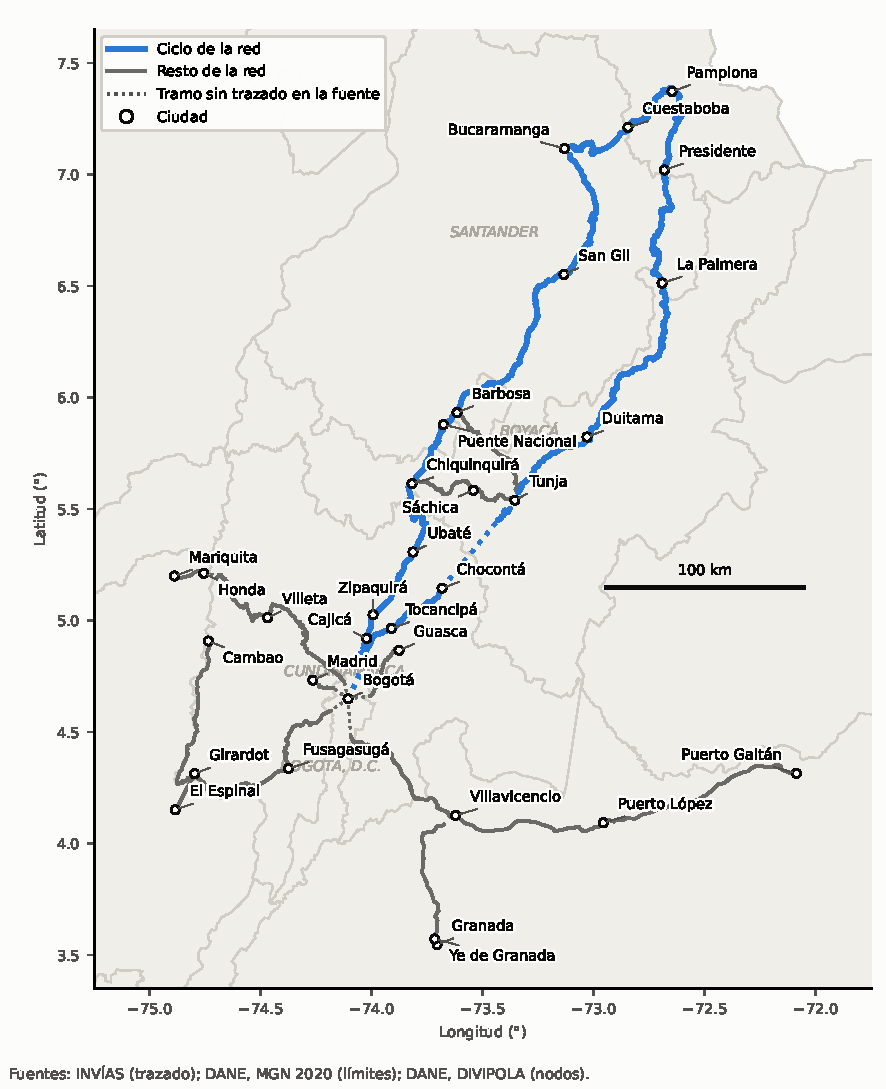
\includegraphics[width=\textwidth]{mapa_red.pdf}
    \caption{Mapa de la red de carga. Fuente: elaboración propia con el
    trazado de INVÍAS, los límites departamentales del DANE~\cite{mgn} y las
    coordenadas DIVIPOLA}
    \label{fig:red}
    \comoleerla{ejes de longitud y latitud; cada línea es el trazado de INVÍAS de un tramo y cada punto una ciudad; el ciclo va en azul, el resto de la red en gris y la línea punteada marca un tramo sin trazado en la fuente.}
{la red tiene 32 ciudades y 32 tramos, 1929.31 km en total; el ciclo, que cierra por Santander, pasa por 15 ciudades.}
{Medido: en 10 de las 32 aristas el trazado queda a más de 5 km de uno de sus nodos (hasta 43.70 km en Chocontá a Tunja) y ahí se dibuja punteado.}

\end{figure}

La Figura~\ref{fig:cobertura} muestra qué aristas tienen dato de riesgo, cuáles tienen peaje y cuáles marca la auditoría geométrica.

\begin{figure}[H]
    \centering
    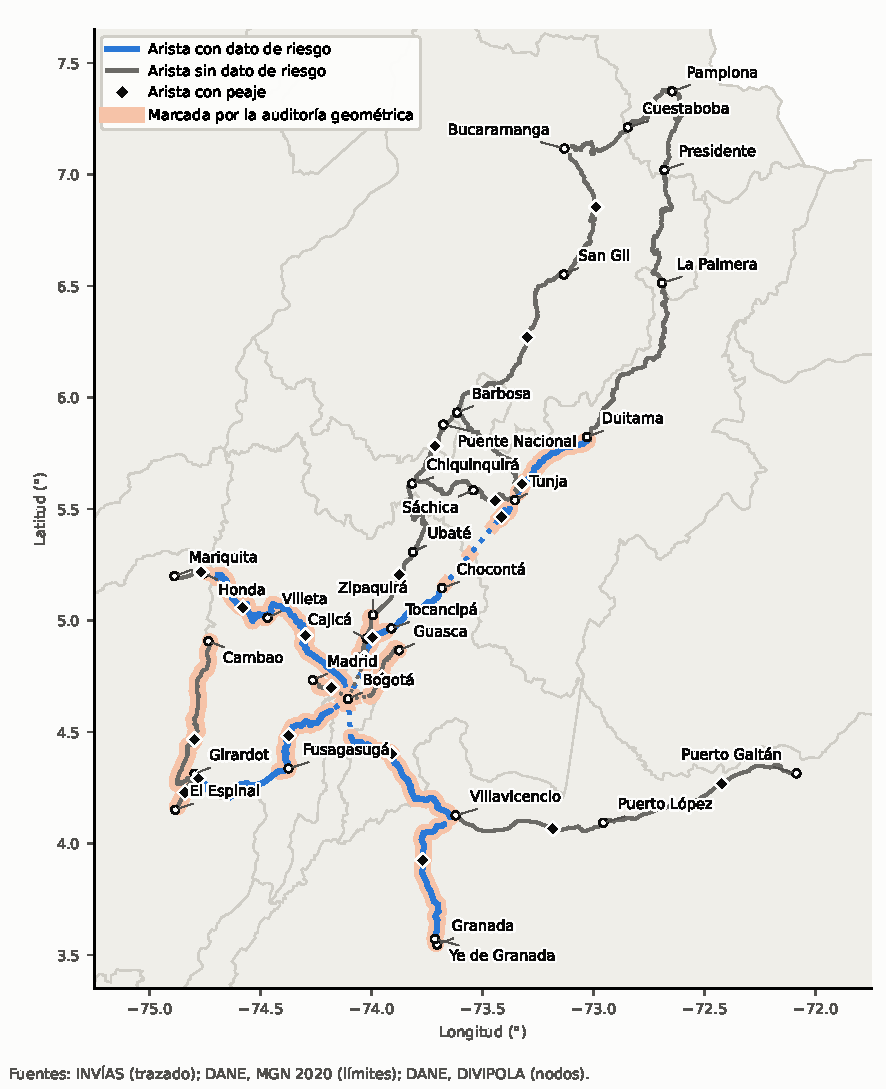
\includegraphics[width=\textwidth]{fig_cobertura.pdf}
    \caption{Cobertura de riesgo y peaje por arista y aristas marcadas por la auditoría. Fuente: elaboración propia}
    \label{fig:cobertura}
    \comoleerla{mapa de la red; el color azul indica dato de riesgo, el rombo negro peaje y el halo naranja claro una arista marcada por la auditoría geométrica.}
{de las 32 aristas, 11 tienen dato de riesgo, 24 tienen peaje y 15 están marcadas por la auditoría.}
{Medido: 21 aristas no tienen dato de riesgo y valen 0 en el costo compuesto.}

\end{figure}

\begin{table}[H]
\centering
\caption{Estadísticas del grafo}
\label{tab:estadisticas}
\begin{tabular}{lr}
\toprule
\textbf{Medida} & \textbf{Valor} \\
\midrule
Nodos (ciudades) & 32 \\
Aristas (tramos) & 32 \\
Grafo conexo & sí \\
Ciclos independientes ($E-V+1$) & 1 \\
Aristas con peaje & 24 de 32 \\
Aristas con dato de riesgo & 11 de 32 \\
Distancia total de la red (km) & 2204.00 \\
$d_{\max}$ (km) & 167.67 \\
$p_{\max}$ (COP) & 41\,600 \\
$r_{\max}$ (GiZScore) & 3.423 \\
\bottomrule
\end{tabular}

\end{table}

\section{Costo compuesto}

El costo de una arista $e$ combina los tres criterios, cada uno normalizado
por su máximo:

\begin{equation}
c(e) = w_1 \frac{d_e}{d_{\max}} + w_2 \frac{p_e}{p_{\max}}
     + w_3 \frac{r_e}{r_{\max}}, \qquad w_1 + w_2 + w_3 = 1
\end{equation}

donde $d_e$ es la distancia, $p_e$ el peaje de categoría III y $r_e$ el
puntaje GiZScore promedio de la arista. No hay un criterio objetivo para
ponderar los tres términos, por lo que se usan pesos iguales
($w_1=w_2=w_3=1/3$); son parámetros ajustables.

\textbf{Normalización por el máximo y no por mín-máx.}
\begin{itemize}
\item La normalización mín-máx resta el mínimo en cada arista, y el costo deja
de ser proporcional a la distancia.
\item La normalización por el máximo conserva esa proporcionalidad: el término
de distancia del costo de una arista sigue siendo proporcional a su longitud.
\item Eso permite contrastarla con la línea recta entre los nodos como
verificación de coherencia de los datos (la carretera no debería ser más corta
que la línea recta; ver la sección de auditoría geométrica).
\end{itemize}

\textbf{Riesgo faltante.} 21 de las 32 aristas no tienen dato de riesgo. No se
imputa ningún valor: tratarlo como 0 sesga las rutas hacia corredores sin
medición. Cada arista guarda el indicador booleano
\texttt{riesgo\_disponible} y se calculan dos variantes:

\begin{itemize}
\item \texttt{peso\_multicriterio}: riesgo faltante igual a 0 (variante
limitada);
\item \texttt{peso\_sin\_riesgo}: sin el término de riesgo, con $w_1$ y $w_2$
renormalizados para sumar 1.
\end{itemize}

\section{Costo monetario}

El costo en pesos de una ruta es el peaje más el costo variable del vehículo,
que es proporcional a los kilómetros:

\begin{equation}
c_{\$}(e) = p_e + d_e \left( \frac{\pi}{\rho} + o \right)
\end{equation}

donde $p_e$ es el peaje de categoría III, $d_e$ la distancia, $\pi$ el precio
del galón de ACPM, $\rho$ el rendimiento en km por galón y $o$ otros costos
variables por km. La Tabla~\ref{tab:insumos-costo} da los insumos, cada uno con
su fuente y su estado.

\begin{table}[H]
\centering
\caption{Insumos del costo monetario}
\label{tab:insumos-costo}
\renewcommand{\arraystretch}{1.2}
\begin{tabular}{|>{\raggedright\arraybackslash}p{3.6cm}|>{\raggedright\arraybackslash}p{2.3cm}|>{\raggedright\arraybackslash}p{4.6cm}|>{\raggedright\arraybackslash}p{2.3cm}|}
\hline
\rowcolor{gray!20} \textbf{Insumo} & \textbf{Valor} & \textbf{Fuente} & \textbf{Estado} \\
\hline
\textbf{Precio del galón de ACPM} & 11\,320 COP & CREG, vigente desde el 2 de octubre de 2026 & verificada \\
\hline
\textbf{Consumo del camión de dos ejes} & 38.69 L por 100 km & UPME, mayo de 2025, Tabla 2.7 (C2G, diésel) & verificada \\
\hline
\textbf{Litros por galón} & 3.785411784 & Definición del galón estadounidense & verificada \\
\hline
\textbf{Otros costos por km} (llantas, mantenimiento, conductor) & 0 COP & Ninguna: no hay tabla descargable por kilómetro & supuesto del equipo \\
\hline
\end{tabular}
\end{table}

Con los insumos verificados el combustible cuesta 1\,157.0 COP por km. El
valor de otros costos por km es un supuesto del equipo (cero, no estimado):
por eso el costo en pesos es un piso, no el costo total del transportador, y
el criterio por defecto de la recomendación sigue siendo el costo compuesto
sin riesgo mientras algún insumo no esté verificado. Los tres insumos
verificados y el supuesto se pueden cambiar por consola
(\texttt{--precio-galon}, \texttt{--rendimiento}, \texttt{--costo-otros-km}),
y la salida rotula esos valores como «dado por el usuario».

\textbf{Costo compuesto total.} Agrega el costo variable como cuarto término
normalizado por su máximo, con cuatro pesos iguales ($w_i=1/4$), que son un
supuesto del equipo:

\begin{equation}
c_T(e) = w_1 \frac{d_e}{d_{\max}} + w_2 \frac{p_e}{p_{\max}}
       + w_3 \frac{r_e}{r_{\max}} + w_4 \frac{v_e}{v_{\max}}
\end{equation}

con $v_e$ el costo variable de la arista. Como $v_e$ es proporcional a $d_e$,
este término pesa lo mismo que la distancia por kilómetro. También se calcula
la variante sin el término de riesgo, con los otros tres pesos renormalizados,
y una variante de sensibilidad que reemplaza el riesgo por la mortalidad de la
ANSV.

\textbf{Umbral de decisión.} Entre la ruta por Bogotá y el desvío por
Santander la decisión por costo en pesos cambia cuando el costo variable por
km alcanza el cociente entre el ahorro de peaje y los kilómetros adicionales:
$70\,600 / 301.84 = 233.9$ COP por km. El valor central (1\,157.0 COP por km)
es unas cinco veces ese umbral, de modo que gana la ruta por Bogotá.

\section{Implementación del agente}

La implementación está en los siguientes módulos de \texttt{src/} y en el
archivo de insumos \texttt{config\_costos.json}:

\begin{itemize}\raggedright
\item \texttt{construir\_red.py}: cruza los conjuntos y genera
\texttt{aristas\_red.json} y \texttt{nodos\_red.json}; el cruce de mortalidad
está en \texttt{cruce\_mortalidad.py}.
\item \texttt{build\_graph.py}: construye el grafo, calcula los pesos y lo
guarda en \texttt{outputs/grafo\_carga.gpickle}.
\item \texttt{agente.py}: clase \texttt{AgenteRutas} con el método
\texttt{calcular\_ruta(origen, destino, criterio, tramos\_bloqueados)}. Los
criterios son \texttt{distancia}, \texttt{peaje}, \texttt{riesgo},
\texttt{compuesto}, \texttt{compuesto\_sin\_riesgo},
\texttt{costo\_operativo}, \texttt{compuesto\_total},
\texttt{compuesto\_total\_sin\_riesgo} y \texttt{compuesto\_mortalidad} (esta
última, de sensibilidad). Usa
\texttt{networkx.shortest\_path} (Dijkstra) sobre el atributo del criterio,
y mide el tiempo con \texttt{time.perf\_counter()} y la memoria pico con
\texttt{tracemalloc}.
\item \texttt{pruebas\_agente.py} y \texttt{pruebas\_costos.py}: pruebas sobre
los 32 nodos y sobre el costo monetario.
\end{itemize}

El parámetro \texttt{tramos\_bloqueados} permite simular un tramo no
disponible, que es la forma de obligar al agente a usar el desvío.

\section{Pruebas}

Las pruebas (\texttt{src/pruebas\_agente.py}) cubren tres grupos de casos y
todas pasan:

\begin{itemize}
\item \textbf{Pares que cruzan el ciclo.} Duitama a Puente Nacional da
352.41 km por Bogotá. Con el tramo Bogotá a Tocancipá bloqueado, da 654.25 km
por Santander. Ambas distancias se comprueban sumando las aristas del JSON.
Con las distancias sin corregir (variante de sensibilidad) las cifras son
414.8 y 668.1 km.
\item \textbf{Pares que no cruzan el ciclo.} Bogotá a Villavicencio, Bogotá a
Granada, Bogotá a Mariquita, Girardot a Cambao, Madrid a Puerto Gaitán y
Chiquinquirá a Tunja. En cada par se enumeraron todos los caminos simples
(existe uno solo) y se comprobó que el agente lo devuelve con los nueve
criterios.
\item \textbf{Entradas inválidas.} Ciudad fuera de la red, criterio
desconocido y destino aislado por un bloqueo producen un error explícito.
\end{itemize}

Las pruebas del costo monetario (\texttt{src/pruebas\_costos.py}) comprueban
que el costo variable de cada ruta es la suma de sus aristas, que el umbral de
233.9 COP por km separa exactamente las dos rutas (por encima gana Bogotá y
por debajo el desvío) y que las opciones de consola con valores inválidos
producen un error explícito.

La Tabla~\ref{tab:criterios} muestra el resultado para Duitama a Puente
Nacional sin bloqueos, con una sola corrida por criterio. Los tiempos y la
memoria son de esa corrida única y se registran solo como referencia.

\begin{table}[H]
\centering
\caption{Duitama a Puente Nacional según el criterio (una corrida)}
\label{tab:criterios}
\small\setlength{\tabcolsep}{2pt}
\renewcommand{\arraystretch}{1.2}
\begin{tabular}{|l|c|r|r|r|r|}
\hline
\rowcolor{gray!20} \textbf{Criterio} & \textbf{Vía} & \textbf{km} & \textbf{Peaje (COP)} & \textbf{Tiempo (ms)} & \textbf{Memoria (KiB)} \\
\hline
\textbf{distancia} & Bogotá & 309.10 & 170\,800 & 0.827 & 3.7 \\
\hline
\textbf{peaje} & Santander & 654.25 & 100\,200 & 0.776 & 3.3 \\
\hline
\textbf{riesgo} & Santander & 654.25 & 100\,200 & 0.618 & 2.9 \\
\hline
\textbf{compuesto} & Santander & 654.25 & 100\,200 & 0.988 & 4.0 \\
\hline
\textbf{compuesto sin riesgo} & Bogotá & 309.10 & 170\,800 & 1.053 & 4.0 \\
\hline
\textbf{costo operativo} & Bogotá & 309.10 & 170\,800 & 0.891 & 3.7 \\
\hline
\textbf{compuesto total} & Bogotá & 309.10 & 170\,800 & 1.088 & 4.0 \\
\hline
\textbf{compuesto total sin riesgo} & Bogotá & 309.10 & 170\,800 & 1.076 & 4.0 \\
\hline
\textbf{compuesto mortalidad} & Bogotá & 309.10 & 170\,800 & 1.063 & 4.0 \\
\hline
\end{tabular}

\comoleerla{filas: los nueve criterios; columnas: vía elegida, distancia, peaje, tiempo y memoria de una corrida del agente.}
{\raggedright por Bogotá (352.41 km, peaje 170\,800 COP) van distancia, compuesto sin riesgo, costo operativo, compuesto total sin riesgo y compuesto mortalidad; por Santander (654.25 km, peaje 100\,200 COP) van peaje, riesgo, compuesto y compuesto total.}
{Medido: la ruta por Santander cuesta 70\,600 COP menos de peaje y sus 7 tramos sin dato de riesgo valen 0.}

\end{table}

Con la distancia, el costo compuesto sin riesgo, el costo operativo (peaje más
combustible) y las variantes del compuesto total sin riesgo y de mortalidad el
agente elige la ruta por Bogotá. Con el peaje, el riesgo, el costo compuesto
con riesgo faltante igual a 0 y el compuesto total elige el desvío por
Santander, y la Tabla~\ref{tab:rutas} explica por qué:

\begin{itemize}
\item El desvío es 301.84 km más largo, pero tiene 70\,600 COP menos de
peaje. En pesos, la ruta por Bogotá cuesta 578\,537 COP (170\,800 de peaje y
407\,737 de combustible) y el desvío 857\,165 COP (100\,200 y 756\,965).
\item El criterio de riesgo lo prefiere porque los siete tramos del desvío no
tienen dato de riesgo y valen 0, no porque se haya medido que es más seguro.
Es el sesgo descrito en la sección del costo compuesto.
\item Sin el término de riesgo, con las distancias sin corregir el costo compuesto era 3.290 por Bogotá y 3.197 por Santander, y ganaba el desvío por Santander; con las distancias corregidas es 3.302 y 3.524, y gana la ruta por Bogotá.
 La corrección de
distancias cambia esa decisión.
\end{itemize}

\begin{table}[H]
\centering
\caption{Las dos rutas reales de Duitama a Puente Nacional}
\label{tab:rutas}
\small
\begin{tabular}{lrr}
\toprule
\textbf{Medida} & \textbf{Ruta corta (Bogotá)} & \textbf{Desvío (Santander)} \\
\midrule
Saltos & 8 & 7 \\
Distancia (km) & 309.10 & 654.25 \\
Peaje total (COP) & 170\,800 & 100\,200 \\
Tramos sin dato de riesgo & 4 & 7 \\
Costo compuesto, riesgo faltante $=0$ & 3.059 & 2.349 \\
Costo compuesto sin riesgo & 3.149 & 3.524 \\
\bottomrule
\end{tabular}

\comoleerla{columnas: la ruta corta por Bogotá y el desvío por Santander; filas: saltos, distancia, peaje, tramos sin riesgo y costos compuestos.}
{el desvío mide 301.84 km más y cuesta 70\,600 COP menos de peaje; el costo compuesto es 3.161 por Bogotá y 2.349 por Santander, y sin riesgo 3.302 y 3.524.}
{Medido: la ruta por Bogotá tiene 4 tramos sin dato de riesgo y el desvío 7, que valen 0 en el costo compuesto.}

\end{table}

La Figura~\ref{fig:casos} compara las dos rutas reales del caso anterior con las cifras de la Tabla~\ref{tab:rutas}.

\begin{figure}[H]
    \centering
    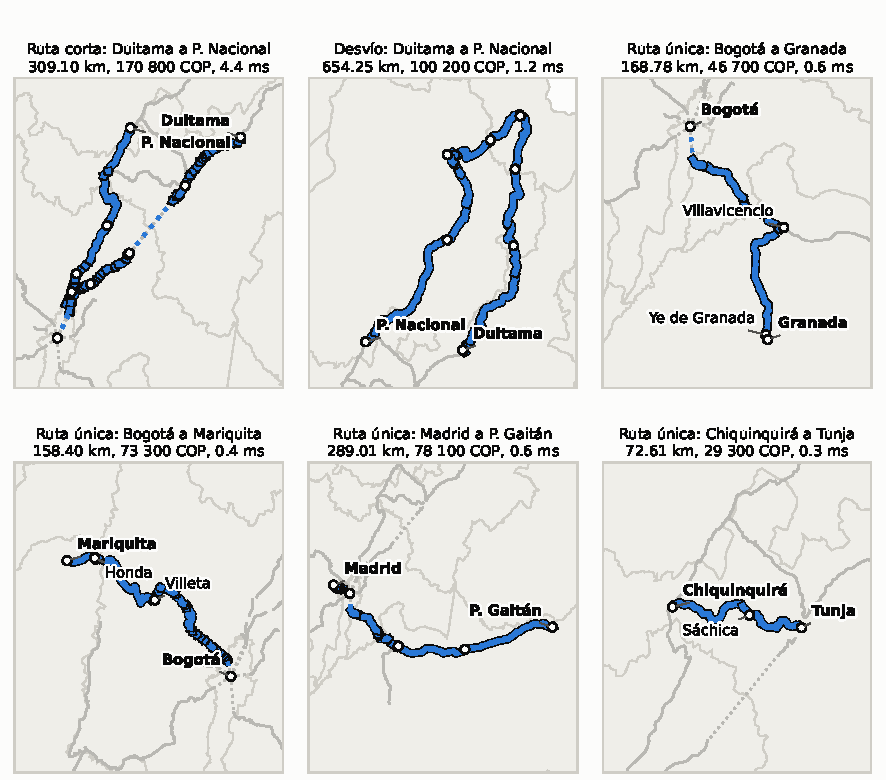
\includegraphics[width=\textwidth]{fig_c1_casos.pdf}
    \caption{Rutas de Duitama a Puente Nacional por Bogotá y por Santander, con distancia, peaje y tiempo. Fuente: elaboración propia}
    \label{fig:casos}
    \comoleerla{un panel por caso de prueba del agente; la línea azul con borde oscuro es la ruta devuelta y la red va en gris; la línea punteada marca un tramo sin trazado en la fuente; el título da la distancia, el peaje y el tiempo de cómputo.}
{los dos primeros paneles son el par que cruza el ciclo, con la ruta corta (352.41 km) y el desvío (654.25 km); los otros cuatro son pares de ruta única.}
{Medido: el tiempo de cómputo de cada caso es el de una sola corrida y es indicativo.}

\end{figure}

\section{Auditoría geométrica de las aristas}

Para comprobar el cruce de datos, cada arista se contrastó con la geometría
del sector de INVÍAS y con la distancia geodésica entre las coordenadas de sus
nodos (Tabla~\ref{tab:auditoria}).
\begin{itemize}
\item Las coordenadas son de la DIVIPOLA del DANE (corte al 30 de diciembre de
2024, descarga del 7 de octubre de 2026).
\item Para Cuestaboba, La Palmera y Yé de Granada no hay punto DANE: la
coordenada se estimó como la unión de los dos tramos de INVÍAS que llegan al
nodo, de modo que en esos tres nodos la coordenada y la geometría de la
carretera no son independientes.
\end{itemize}

\textbf{Hallazgos:}

\begin{itemize}
\item \textbf{Chocontá a Tunja truncada en la fuente, corregida con las
progresivas.}
\begin{itemize}
\item El sector registra 17.69 km y Chocontá queda a 43.70 km de su geometría;
con ese valor la razón carretera/geodésica era 0.3106.
\item Ambos sectores pertenecen a la ruta 55 y al mismo tramo (5501), y sus
progresivas (Chocontá en PR 59.0 y Tunja en PR 120.0) dejan un intervalo de
49.1 km sin registro; la diferencia de progresivas es 61.0 km, que es la
distancia vigente de la arista (razón 1.071). La longitud registrada de 17.69
km se conserva como variante de sensibilidad.
\item La regla exige que la distancia por progresivas no sea menor que la
geodésica (56.96 km); se cumple.
\item Con esta corrección la ruta corta de Duitama a Puente Nacional mide
352.41 km y ya no es un valor acotado inferiormente.
\end{itemize}
\item \textbf{Bogotá a Mosquera excluida.} El sector asignado pertenecía a
la Troncal del Eje Cafetero, a unos 160 km de Mosquera; el nodo se excluyó
(ver la sección de datos y metodología). La auditoría de esta sección ya no
incluye esa arista.
\item \textbf{Entrada urbana a Bogotá.} Las geometrías que salen de Bogotá
empiezan en el límite urbano, a entre 8.50 y 19.06 km de la coordenada del
municipio. Es una limitación de la fuente y no se corrige.
\item \textbf{Siete aristas con la carretera más corta que la línea recta}
(razón menor que 1, ya con la corrección de doble calzada): Madrid a Bogotá
(0.458), Bogotá a Tocancipá (0.537), Cajicá a Zipaquirá (0.749), Granada a Yé
de Granada (0.798), El Espinal a Girardot (0.948), Bogotá a Guasca (0.993) y
Tunja a Duitama (0.999). Varias se deben a la entrada urbana a Bogotá.
\item \textbf{Doble calzada digitalizada, corregida.}
\begin{itemize}
\item En 9 registros la longitud registrada es entre 1.7 y 2.3 veces el tramo
entre progresivas, porque la geometría contiene ambas calzadas (Tunja a
Duitama, Tocancipá a Chocontá, Cajicá a Zipaquirá, Bogotá a Villeta, Madrid a
Bogotá, Bogotá a Fusagasugá, Fusagasugá a Girardot, Bogotá a Tocancipá y un
registro de San Gil a Bucaramanga).
\item La regla se fijó de antemano (si la razón está entre 1.7 y 2.3 se usa el
tramo entre progresivas; si no, la longitud registrada) y se verificó con una
segunda medida oficial: en los 9 registros la diferencia relativa entre el
tramo entre progresivas y el camino a lo largo de la geometría es a lo sumo
0.123 (límite 0.15).
\end{itemize}
\item \textbf{Registros con patrón no estándar.} Quedan fuera de la banda y
conservan la longitud registrada: Bogotá a Cajicá (razón 3.18), El Espinal a
Girardot (1.21) y el registro del Río Ocoa (9.77). Chocontá a Tunja (1.49) se
resuelve aparte, con las progresivas del corredor.
\end{itemize}

La regla se fijó de antemano y no se ajustó ninguna distancia para obtener un
resultado determinado: el principio es corregir solo errores demostrables, con
datos oficiales.

La Figura~\ref{fig:coherencia} contrasta, arista por arista, la distancia por carretera con la geodésica.

\begin{figure}[H]
    \centering
    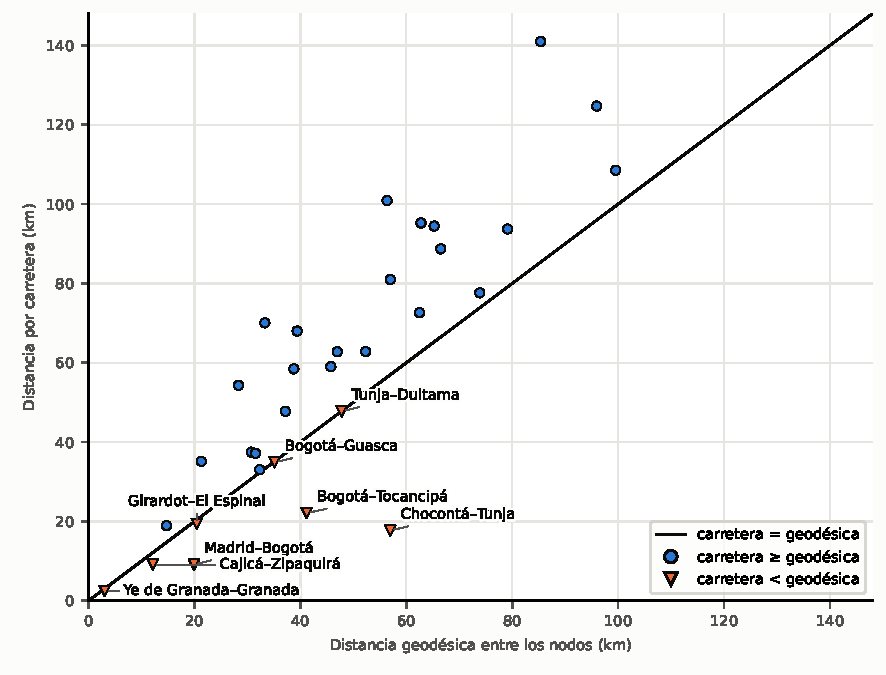
\includegraphics[width=\textwidth]{fig_c1_coherencia.pdf}
    \caption{Distancia por carretera contra distancia geodésica de las 32 aristas. Fuente: elaboración propia}
    \label{fig:coherencia}
    \comoleerla{cada punto es una de las 32 aristas: distancia geodésica en el eje horizontal y distancia por carretera en el vertical; la recta es y = x.}
{24 aristas tienen carretera igual o mayor que la geodésica y 8 la tienen menor.}
{Medido: la menor razón es 0.3106 en Chocontá a Tunja; las aristas bajo la recta son las que la auditoría marca por carretera menor que la geodésica.}

\end{figure}

\subsection{Aristas marcadas por la auditoría}

Las 32 aristas auditadas están en \texttt{outputs/auditoria\_aristas.csv}; la
Tabla~\ref{tab:auditoria} lista las que tienen alguna marca, con la distancia
por carretera del grafo, la geodésica, su razón y la mayor separación entre un
extremo de la geometría del sector y su nodo (Ext.), todas en km. Marcas:
\begin{itemize}
\item[A] Carretera menor que la geodésica.
\item[B] Extremo a más de 5 km del nodo.
\item[C] Nodo a más de 5 km de la geometría.
\item[D] Registro mayor que 1.5 veces el camino de su geometría.
\item[E] Geometría sin camino entre extremos.
\end{itemize}

\begin{table}[H]
\centering
\caption{Aristas marcadas por la auditoría geométrica}
\label{tab:auditoria}
\small\setlength{\tabcolsep}{3pt}
\begin{longtable}{lrrrrl}
\caption{Auditoría geométrica de las aristas}\label{tab:auditoria}\\
\toprule
\textbf{Arista} & \textbf{Carr.} & \textbf{Geod.} & \textbf{Razón} & \textbf{Ext.} & \textbf{Marcas} \\
\midrule
\endhead
Bogotá -- Tocancipá & 38.37 & 41.19 & 0.932 & 18.90 & A,B,C,D \\
Tocancipá -- Chocontá & 66.49 & 32.31 & 2.058 & 1.26 & D \\
Chocontá -- Tunja & 17.69 & 56.96 & 0.311 & 43.70 & A,B,C \\
Tunja -- Duitama & 94.18 & 47.78 & 1.971 & 4.17 & D \\
Barbosa -- Tunja & 62.83 & 52.31 & 1.201 & 4.24 & --- \\
Chiquinquirá -- Sáchica & 37.46 & 30.74 & 1.218 & 4.55 & --- \\
Sáchica -- Tunja & 35.15 & 21.28 & 1.652 & 4.55 & --- \\
Bogotá -- Cajicá & 37.18 & 31.51 & 1.180 & 19.02 & B,C,D \\
Cajicá -- Zipaquirá & 18.69 & 12.15 & 1.539 & 2.14 & D \\
Zipaquirá -- Ubaté & 47.76 & 37.16 & 1.285 & 1.26 & --- \\
Ubaté -- Puente Nacional & 94.48 & 65.26 & 1.448 & 0.84 & --- \\
Madrid -- Bogotá & 19.46 & 19.91 & 0.978 & 8.96 & A,B,C,D \\
Bogotá -- Guasca & 34.88 & 35.12 & 0.993 & 11.17 & A,B,C \\
Bogotá -- Villavicencio & 93.72 & 79.15 & 1.184 & 19.06 & B,C \\
Villavicencio -- Ye de Granada & 72.63 & 62.48 & 1.163 & 2.08 & E \\
Ye de Granada -- Granada & 2.43 & 3.04 & 0.798 & 0.86 & A \\
Villavicencio -- Puerto López & 77.62 & 73.88 & 1.051 & 3.09 & --- \\
Puerto López -- Puerto Gaitán & 108.55 & 99.54 & 1.091 & 1.40 & --- \\
Bogotá -- Villeta & 167.67 & 57.00 & 2.942 & 8.50 & B,C,D \\
Villeta -- Honda & 58.45 & 38.76 & 1.508 & 7.56 & B,C \\
Honda -- Mariquita & 18.95 & 14.71 & 1.288 & 1.93 & --- \\
Bogotá -- Fusagasugá & 111.76 & 45.75 & 2.443 & 10.39 & B,C,D \\
Fusagasugá -- Girardot & 111.39 & 46.95 & 2.373 & 5.00 & D \\
Girardot -- El Espinal & 19.36 & 20.42 & 0.948 & 3.07 & A \\
Girardot -- Cambao & 88.71 & 66.51 & 1.334 & 9.98 & B,E \\
Puente Nacional -- San Gil & 124.72 & 95.97 & 1.300 & 0.84 & --- \\
San Gil -- Bucaramanga & 109.14 & 62.77 & 1.739 & 4.13 & --- \\
Bucaramanga -- Cuestaboba & 70.06 & 33.29 & 2.105 & 3.93 & --- \\
Cuestaboba -- Pamplona & 54.31 & 28.32 & 1.918 & 1.68 & --- \\
Pamplona -- Presidente & 68.00 & 39.38 & 1.727 & 1.32 & --- \\
Presidente -- La Palmera & 100.90 & 56.37 & 1.790 & 0.13 & --- \\
La Palmera -- Duitama & 141.01 & 85.38 & 1.651 & 2.19 & --- \\
\bottomrule
\end{longtable}

\comoleerla{filas: las aristas marcadas por la auditoría; columnas: distancia por carretera, geodésica, su razón, la mayor separación entre un extremo del trazado y el nodo, y las marcas A a E.}
{15 de 32 aristas tienen alguna marca: 8 con carretera menor que la línea recta (A), 10 con el trazado lejos de un nodo (B) y 2 sin camino entre extremos (E).}
{Medido: 7 de las aristas con extremo lejos salen de Bogotá, con el trazado a entre 8.50 y 19.06 km del nodo.}

\end{table}

\section{Registro de decisiones de diseño}

\begin{table}[H]
\centering
\caption{Decisiones de diseño y su motivo}
\label{tab:decisiones}
\small
\renewcommand{\arraystretch}{1.2}
\begin{tabular}{|>{\raggedright\arraybackslash}p{4.4cm}|>{\raggedright\arraybackslash}p{9cm}|}
\hline
\rowcolor{gray!20} \textbf{Decisión} & \textbf{Motivo} \\
\hline
\textbf{Cambio de dominio de TransMilenio a carga interurbana} & El profesor señaló que el tema anterior es básico y lo presentan muchos grupos \\
\hline
\textbf{Extender la red de 27 a 33 nodos} & Un árbol tiene una única ruta posible entre cada par de ciudades \\
\hline
\textbf{Excluir Mosquera (33 a 32 nodos)} & Su sector pertenece a otra región, no hay sector oficial de reemplazo y era una hoja \\
\hline
\textbf{Chocontá a Tunja por progresivas (61.0 km)} & El sector registrado (17.69 km) está truncado; las progresivas oficiales del mismo corredor y tramo dan 61.0 km, no menos que la geodésica (56.96 km). La longitud registrada queda como sensibilidad \\
\hline
\textbf{Regla de doble calzada digitalizada} & En 9 registros la longitud es entre 1.7 y 2.3 veces el tramo entre progresivas; la regla se fijó de antemano y se verificó con la geometría \\
\hline
\textbf{Cruce de distancia por \texttt{sector} exacto} & Un mismo código de tramo agrupa subtramos de longitud distinta \\
\hline
\textbf{Normalización por el máximo} & Conserva la proporcionalidad con la distancia \\
\hline
\textbf{Pesos iguales} & No hay criterio objetivo para ponderar los tres términos (ni, en el compuesto total, los cuatro); son un supuesto del equipo \\
\hline
\textbf{Costo monetario con insumos rotulados} & Precio del galón (CREG) y consumo (UPME) son verificados; otros costos por km queda en 0 como supuesto del equipo, sin estimarlo \\
\hline
\textbf{Mortalidad de la ANSV solo como sensibilidad} & Cubre 16 de 32 aristas, pero no reproduce el orden del puntaje GiZScore (Spearman $-0.033$) \\
\hline
\textbf{Riesgo faltante sin imputar} & Imputar 0 sesga hacia corredores sin medición; se guardan dos variantes \\
\hline
\textbf{Tarifas de peaje de la descarga del 6 de octubre de 2026} & Son las de la fuente oficial vigente; 10 de las 24 tarifas cambiaron respecto de una descarga anterior \\
\hline
\textbf{Tabla explícita de peajes} & Evita emparejar por texto y falla si el peaje no aparece exactamente una vez \\
\hline
\end{tabular}
\end{table}

\section{Limitaciones}

\begin{itemize}
\item \textbf{Riesgo incompleto.} Solo 11 de las 32 aristas tienen dato de
puntaje GiZScore. En las otras 21 el riesgo no se midió, y la variante con
riesgo igual a 0 sesga las rutas hacia ellas. El atributo de mortalidad cubre
16 aristas, pero no reproduce el orden del puntaje y solo sirve como
sensibilidad.
\item \textbf{Costo monetario parcial.} Solo el combustible está respaldado por
fuentes; los demás costos variables (llantas, mantenimiento, conductor) valen
0 como supuesto del equipo, de modo que el costo en pesos es un piso. Los
pesos del compuesto total son también un supuesto.
\item \textbf{Riesgo por corredor.} El dato no distingue subtramos. Los
fallecidos y los puntos críticos son totales del corredor y se repiten en
cada arista que lo compone; cuando una arista pertenece a dos corredores se
promedia el puntaje y se suman fallecidos y puntos.
\item \textbf{Vigencia de las tarifas.} Las tarifas de peaje se actualizan
cada año; los costos corresponden a la descarga del 6 de octubre de 2026.
\item \textbf{Artefacto de doble calzada.} Bogotá a Villeta reportaba
167.67 km por la doble calzada digitalizada; la corrección deja 81.00 km. Los
registros con patrón no estándar conservan la longitud registrada.
\item \textbf{Hallazgos de la auditoría geométrica.} Las distancias son las
del dato oficial, salvo la doble calzada y Chocontá a Tunja, que se
corrigieron con datos oficiales. Las distancias desde Bogotá excluyen la
entrada urbana, para la cual no se halló una fuente aceptable. Ver la sección
de auditoría geométrica.
\item \textbf{Alcance.} La red excluye la rama Villavicencio, Barranca de
Upía y Yopal, y el nodo Mosquera, y tiene un solo ciclo. Los pares que no lo
cruzan tienen una única ruta posible.
\item \textbf{Mediciones.} El tiempo y la memoria de la
Tabla~\ref{tab:criterios} provienen de una sola corrida.
\item \textbf{Mapa.} El fondo departamental está generalizado a unos 330 m y
no sirve para medir distancias. Los tramos punteados no tienen trazado en la
fuente: la geometría de INVÍAS queda a más de 5 km de uno de sus nodos.
\end{itemize}

\renewcommand{\refname}{Referencias}
\addcontentsline{toc}{section}{Referencias}

\begin{thebibliography}{9}

\bibitem{redvial}
INVÍAS. (2026). \textit{Red Vial}. Datos Abiertos Colombia.
\url{https://www.datos.gov.co/Transporte/Red-Vial/ie7y-asdn}

\bibitem{peajes}
INVÍAS. (2026). \textit{Peajes}. Datos Abiertos Colombia.
\url{https://www.datos.gov.co/Transporte/Peajes/68qj-5xux}

\bibitem{siniestralidad}
Agencia Nacional de Seguridad Vial. (2026). \textit{Sectores críticos de
siniestralidad vial}. Datos Abiertos Colombia.
\url{https://www.datos.gov.co/Transporte/SECTORES-CRITICOS-DE-SINIESTRALIDAD-VIAL/rs3u-8r4q}

\bibitem{mgn}
Departamento Administrativo Nacional de Estadística. (2020).
\textit{Nivel de información Departamento del Marco Geoestadístico Nacional
(MGN), versión 2020}. Datos Abiertos Colombia (descargado el 7 de octubre de
2026). \url{https://www.datos.gov.co/d/jjim-6r88}

\end{thebibliography}

\end{document}
